% ****** Start of file apssamp.tex ******
%
%   This file is part of the APS files in the REVTeX 4.2 distribution.
%   Version 4.2a of REVTeX, December 2014
%
%   Copyright (c) 2014 The American Physical Society.
%
%   See the REVTeX 4 README file for restrictions and more information.
%
% TeX'ing this file requires that you have AMS-LaTeX 2.0 installed
% as well as the rest of the prerequisites for REVTeX 4.2
%
% See the REVTeX 4 README file
% It also requires running BibTeX. The commands are as follows:
%
%  1)  latex apssamp.tex
%  2)  bibtex apssamp
%  3)  latex apssamp.tex
%  4)  latex apssamp.tex
%
\documentclass[%
 reprint,
%superscriptaddress,
%groupedaddress,
%unsortedaddress,
%runinaddress,
%frontmatterverbose, 
%preprint,
%preprintnumbers,
%nofootinbib,
%nobibnotes,
%bibnotes,
 amsmath,amssymb,
 aps,
%pra,
%prb,
%rmp,
%prstab,
%prstper,
%floatfix,
]{revtex4-2}

\usepackage{listings}
\usepackage{xcolor}

% Optional: Define a style for your Python code
\lstdefinestyle{pythonstyle}{
    language=Python,
    backgroundcolor=\color{gray!10},
    commentstyle=\color{green!60!black}\textit,
    keywordstyle=\color{blue}\bfseries,
    stringstyle=\color{red},
    basicstyle=\ttfamily\footnotesize,
    breaklines=true,
    showstringspaces=false,
    numbers=left,
    numberstyle=\tiny\color{gray},
    frame=single,
    framerule=0pt,
    title=\lstlistingname{}: \texttt{whittle\_likelihood\_arrays} and \texttt{multivariate\_psplines\_model}
}

\usepackage{graphicx}% Include figure files
\usepackage{dcolumn}% Align table columns on decimal point
\usepackage{bm}% bold math
%\usepackage{hyperref}% add hypertext capabilities
%\usepackage[mathlines]{lineno}% Enable numbering of text and display math
%\linenumbers\relax % Commence numbering lines

%\usepackage[showframe,%Uncomment any one of the following lines to test 
%%scale=0.7, marginratio={1:1, 2:3}, ignoreall,% default settings
%%text={7in,10in},centering,
%%margin=1.5in,
%%total={6.5in,8.75in}, top=1.2in, left=0.9in, includefoot,
%%height=10in,a5paper,hmargin={3cm,0.8in},
%]{geometry}


\usepackage{xcolor}




\newcommand{\avi}[1]{\textcolor{orange}{[Avi: #1]}}
\newcommand{\RM}[1]{\textcolor{red}{[RM: #1]}}
\newcommand{\kl}[1]{\textcolor{violet}{Kate : #1}}
\newcommand{\KJ}[1]{\textcolor{teal}{KJ : #1}}
\newcommand{\NC}[1]{\textcolor{green}{NC : #1}}
\newcommand{\pmr}[1]{\textcolor{blue}{[Patricio: #1]}}
\newcommand{\jliu}[1]{\textcolor{blue}{[Jianan: #1]}}

\newcommand{\citeme}{\textcolor{red}{[CITEME]}}


\newcommand{\vect}[1]{\boldsymbol{#1}}
\renewcommand{\d}{{\bf d}}
\newcommand{\bnu}{\mbox{\boldmath $\nu$}}
\newcommand{\bmu}{\mbox{\boldmath $\mu$}}
\newcommand{\bxi}{\mbox{\boldmath $\xi$}}
\newcommand{\bphi}{ \phi}
\newcommand{\btheta}{\mbox{\boldmath $\theta$}}
\newcommand{\bdelta}{\mbox{\boldmath $\delta$}}
\newcommand{\balpha}{\mbox{\boldmath $\alpha$}}
\renewcommand{\S}{{\bf S}}
\newcommand{\A}{{\bf A}}
\newcommand{\Y}{{\bf Y}}
\newcommand{\Z}{{\bf Z}}

\newcommand{\Sn}{\ensuremath{S_n^{\mathrm{GP}}}}
\newcommand{\eqq}{\ensuremath{\!\mathrel{\scalebox{0.7}{=}}\!}}
\newcommand{\tmes}{\ensuremath{{\mkern-2mu\times\mkern-2mu}}}
\newcommand{\ex}[1]{\ensuremath{\tmes10^{\text{-}#1}}}



\newcommand{\project}[1]{\textsf{#1}}

\newcommand{\python}{\project{Python}}
\newcommand{\scipy}{\project{scipy}}
\newcommand{\jupyterbook}{\project{Jupyter Book}}
\newcommand{\numpy}{\project{numpy}}
\newcommand{\pandas}{\project{pandas}}
\newcommand{\matplotlib}{\project{matplotlib}}
\newcommand{\hyperopt}{\project{HyperOpt}}
\newcommand{\tensorflowProb}{\project{TensorFlow Probability}}

\newcommand{\tr}{\mbox{tr}}
\newcommand{\I}{\mbox{{\bf I}}}
\newcommand{\e}{{\rm e}}
\newcommand{\M}{{\bf M}}
\newcommand{\U}{{\bf U}}
\renewcommand{\u}{\mathbf {u}}
\renewcommand{\v}{{\bf v}}





\begin{document}

\preprint{APS/123-QED}

\title{Multivariate p-splines}

\author{NZ Gravity}
%  \altaffiliation[Also at ]{Physics Department, XYZ University.}%Lines break automatically or can be forced with \\
% \author{Second Author}%
%  \email{Second.Author@institution.edu}
% \affiliation{%
%  Authors' institution and/or address\\
%  This line break forced with \textbackslash\textbackslash
% }%

% \collaboration{MUSO Collaboration}%\noaffiliation

% \author{Charlie Author}
%  \homepage{http://www.Second.institution.edu/~Charlie.Author}
% \affiliation{
%  Second institution and/or address\\
%  This line break forced% with \\
% }%
% \affiliation{
%  Third institution, the second for Charlie Author
% }%
% \author{Delta Author}
% \affiliation{%
%  Authors' institution and/or address\\
%  This line break forced with \textbackslash\textbackslash
% }%


\date{\today}% It is always \today, today,
             %  but any date may be explicitly specified

\begin{abstract}

This article extends the p-spline method to the multivariate case.

\end{abstract}

\keywords{gravitational waves, CSD estimation, P-splines, LISA}

\maketitle

%\tableofcontents

\section{\label{sec:intro}Introduction}

LISA will provide three correlated data streams from time-delay interferometry combinations. 
Accurate characterization of the noise spectral density matrix $\mathbf{S}(f)$ is essential for optimal signal detection and parameter estimation in this multivariate setting.

LISA data exhibits several characteristics that challenge conventional spectral estimation methods: frequency-dependent cross-correlations between channels, non-stationary noise properties due to orbital motion, and overlapping astrophysical signals across the millihertz band. 
The P-spline approach addresses these challenges through XYZ.

The estimated spectral density matrices serve multiple roles in LISA data analysis. 
They provide noise weighting for matched filtering operations, enable detection of instrumental anomalies through spectral monitoring, and support background characterization for targeted source analyses. 
The Bayesian framework naturally propagates spectral uncertainties to downstream parameter estimation procedures.

Integration with LISA's global analysis pipeline requires spectral estimates across multiple time scales, from hourly monitoring to months-long campaigns. 
The computational efficiency of the P-spline method, with $O(N k)$ scaling where $k \ll N$, makes such continuous analysis feasible. 
\avi{Im guessing its O(nk), id like to actually show it.}

Implementation of this methodology is expected to improve LISA's detection sensitivity through more accurate noise characterization and reduce systematic errors in parameter estimation by properly accounting for inter-channel correlations. 
These improvements directly impact LISA's primary science objectives, including the detection of massive black hole mergers, galactic binary systems, and potential primordial gravitational wave backgrounds.


\section{Multivariate P-splines}


\subsection{Likelihood}
Assume we are given a time series of gravitational wave observations of length $n$ from $p$ channels. To set notation,
let $\Z=(\Z_1,\ldots,\Z_n)^ \intercal\in  \mathbb{R}^{n\times p}$ be a $p$-dimensional stationary, mean-zero time series, sampled at time intervals $\Delta_t=1/(2f_{Ny})$, i.e., \textcolor{blue}{$\Z_\ell=\Z(\ell\Delta_t)\in \mathbb{R}^p$ for $l=1,\ldots,n$}, where $f_{Ny}$ is the Nyquist frequency, for a total observation time of $T$ with a total of $n=T/\Delta_t$ sampled values for each of the $p$ dimensions. The frequency resolution, \(\Delta_f\), is given by
\begin{align}
\Delta_f = \frac{1}{n \Delta_t} = \frac{1}{T}\, .
\end{align}
Let $\d_k=(d_1(f_k), d_2(f_k), \ldots, d_p(f_k))^T$ be the \ac{DFT} of $\Z$ given by
\begin{align}
\d(f_k) = \Delta_t\sum_{t=1}^{n} \Z_t\exp \left(-2\pi i \frac{k}{n} t \right)\, ,
\end{align}
where $f_k= k \Delta_f= k/({n\Delta_t})=k /{T}$ for $k=1,\ldots, N$, and $N = n/2$ if n is even, $N = (n-1)/2$ if n is odd. 
%\textcolor{green}{RM: This should have read spectral density instead of Fourier transform. I don't think we need this sentence any more as the referee has asked to explicitly define the PSD. Also, if we keep this sentence, it should go after the definition of the spectral density.}
%
%Due to the normalizing and decorrelating properties of the Fourier transform, 
For stationary time series with absolutely summable autocovariances, i.e., $\sum_{h=1}^\infty\gamma_{lm}(h)<\infty$, the discrete Fourier coefficients $\d(f_k)$ %(multiplied by $1 / \sqrt{n}$)
are asymptotically independent and have a complex Gaussian distribution with mean zero and  covariance matrix $T\, \S(f_k)$ with  the continuous two-sided spectral density matrix 
\[\S(f)=\frac{1}{2f_{Ny}}
\sum_{\ell=-\infty}^{\infty} \Gamma(\ell \Delta_t) \exp \left(-2\pi i f \ell\Delta_t \right),\]} %
the Fourier transform of the time-invariant autocovariance function $\Gamma(h)=\left( \gamma_{lm}(h)\right)=\mathbb{E}(\Z_{t}\Z_{t+h}^\intercal)$ that in turn defines the Toeplitz covariance matrix of $\Z$. This asymptotic Gaussian distribution is the basis of the multivariate Whittle likelihood approximation in the frequency domain, expressed as


%Let $\bold{d}(f_j) = [d_1(f_j), d_2(f_j), \ldots, d_p(f_j)]^T$ denote the $p$-dimensional complex Fourier coefficient vector at frequency $f_j$, where $d_k(f_j)$ represents the discrete Fourier transform of the $k$-th channel of the multivariate time series.

The multivariate log-Whittle likelihood is given by
\begin{align}\label{eq:Whittle likelihood}
 \mathcal{L}(\d|\S) &\propto  \prod_{k=1}^{N} \det(\S(f_k))^{-1} \times \nonumber \\
 & \exp\left(-\frac{1}{T}\d(f_k)^* \S(f_k)^{-1} \d(f_k)\right)
\end{align}
where $\d(f_k)^*$ is the conjugate transpose of the $\d(f_k)$ and $\S(f_k)$ is a $p \times p$ Hermitian positive semidefinite spectral density matrix at each $f_k$. 

%\begin{align}
%L(\bold{d}|\bold{S}) = -\sum_{j=1}^{N} \left\{ \log |\bold{S}(f_j)| + \frac{1}{T}\bold{d}(f_j)^* \bold{S}(f_j)^{-1} \bold{d}(f_j)\right\},    
%\end{align}
%where $\bold{d}(f_j)^*$ is the conjugate transpose and $\bold{S}(f_j)$ is the $p %\times p$ Hermitian positive definite spectral density matrix at frequency $f_j$.

\subsection{Parameterization using the Cholesky Decomposition}
Following the approach of \citet{RosenOri2007Aeom,Hu2023}, we parameterize the inverse spectral density matrix using its Cholesky decomposition. Specifically, we write $\bold{S}(f_k)^{-1} = \bold{T}(f_k)^* \bold{D}(f_k)^{-1} \bold{T}(f_k)$, where $\bold{D}(f_k)$ is a diagonal matrix with positive diagonal elements $\delta_{1k}^2, \delta_{2k}^2, \ldots, \delta_{pk}^2$ and
\begin{align}
\bold{T}(f_k) = \begin{pmatrix}
1 & 0 & 0 & \cdots & 0 \\
-\theta_{21}(f_k) & 1 & 0 & \cdots & 0 \\
-\theta_{31}(f_k) & -\theta_{32}(f_k) & 1 & \ddots & \vdots \\
\vdots & \vdots & \ddots & \ddots & 0 \\
-\theta_{p1}(f_k) & -\theta_{p2}(f_k) & \cdots & -\theta_{p,p-1}(f_k) & 1
\end{pmatrix}
\end{align}
is a $p \times p$ complex unit lower triangular matrix with $\theta_{il}(f_k)$ representing the complex-valued off-diagonal elements for $i > l$.

This parameterization allows us to rewrite the likelihood as
\begin{align}
L(\bold{u}|\delta,\theta) = \sum_{k=1}^{N} \left\{ \sum_{j=1}^{p} \log \delta_{jk}^{-2} - \left|\bold{u}(f_k)\right|^2 \right\},
\end{align}
where $\bold{u}(f_k) = \bold{T}(f_k) \bold{D}(f_k)^{-1/2} \bold{d}(f_k)$ represents the whitened data, and $|\cdot|^2$ denotes the squared magnitude.

\textcolor{red}{
This parameterization allows us to rewrite the likelihood as the product of $p$ likelihoods $L_j$ depending on $\btheta_j,\bdelta_j$, for $j=1,\ldots,p$,
\textcolor{red}{\begin{align}
 \mathcal{L}(\d|\S)
 \propto \prod_{j=1}^{p} \mathcal{L}_j(\d_j,\d_{<j}|{\btheta_j,\bdelta_j})
 \label{eq:likelihood}
\end{align}}
where
\begin{align}
\mathcal{L}_j(&\d_j,\d_{<j}|\btheta_j,\bdelta_j) \propto \nonumber \\
&  \prod_{k=1}^{N} \delta_{jk}^{-2} \exp \left(\frac{-\left|d_j(f_k)-\sum_{l=1}^{j-1}\theta_{jl}^{(k)}d_l(f_k) \right|^2}{T\delta_{jk}^2} \right)
\label{eq:likelihoodj}
\end{align}%
and $\d_{<j}$ denotes the data of channels preceding the $j$th channel, the parameters $\btheta_j,\bdelta_j$ represent the set of $\theta_k$ and $\delta_k$ for the $j$th component of the multivariate time series, $\theta_{jl}^{(k)}$ represents the corresponding element in the matrix $T_k$ for any $j>l$, and $\theta_{jl}^{(k)} = 1$ when $j=l$, $d_j(f_k)$ denotes the Fourier coefficient of the $j$th component, and $\d_j=(d_j(f_1),\ldots,d_j(f_N))^\intercal$.
Explicitly, if we have 3 channels as in the LISA case, we have 3 independent likelihoods ${\mathcal L}_j$ that depend on subvectors $\bdelta_1$, $(\bdelta_2,\btheta_{21})$, and $(\bdelta_3,\btheta_{31},\btheta_{32})$ of the total parameter vector:
\begin{align}
\mathcal{L}_1(&\d_1|\bdelta_1) \propto \nonumber \\
&  \prod_{k=1}^{N} \delta_{1k}^{-2} \exp \left(\frac{-\left|d_1(f_k) \right|^2}{T\delta_{1k}^2} \right)
\label{eq:likelihood1}
\end{align}%
\begin{align}
\mathcal{L}_2(&\d_1,\d_2|\btheta_{21},\bdelta_2) \propto \nonumber \\
&  \prod_{k=1}^{N} \delta_{2k}^{-2} \exp \left(\frac{-\left|d_2(f_k)-\theta_{21}^{(k)}d_1(f_k) \right|^2}{T\delta_{2k}^2} \right)
\label{eq:likelihood2}
\end{align}%
\begin{align}
\mathcal{L}_3(&\d_1,\d_2,\d_3|\btheta_{31},\btheta_{32}\bdelta_3) \propto \nonumber \\
&  \prod_{k=1}^{N} \delta_{3k}^{-2} \exp \left(\frac{-\left|d_3(f_k)-\theta_{31}^{(k)}d_1(f_k) -\theta_{32}^{(k)}d_2(f_k)\right|^2}{T\delta_{3k}^2} \right)
\label{eq:likelihood3}
\end{align}%
This means, we can run an MCMC chain for each posterior of $\bdelta_1$, $(\bdelta_2,\btheta_{21})$, and $(\bdelta_3,\btheta_{31},\btheta_{32})$ separately and in parallel which should reduce the computation time.
}


\subsection{P-spline Modeling}
We model the frequency-dependent parameters using penalized B-splines. Specifically, we represent:
\begin{align}
\log \delta_{kj}^2 &= \sum_{m=1}^{M_k} B_m(f_j) w_{k,m}^{(\delta)} \label{eq:delta_spline}\\
\Re[\theta_{kl}(f_j)] &= \sum_{m=1}^{M_{kl}} B_m(f_j) w_{kl,m}^{(\Re)} \label{eq:theta_re_spline}\\
\Im[\theta_{kl}(f_j)] &= \sum_{m=1}^{M_{kl}} B_m(f_j) w_{kl,m}^{(\Im)} \label{eq:theta_im_spline}
\end{align}
where $B_m(f_j)$ are B-spline basis functions evaluated at frequency $f_j$, $M_k$ and $M_{kl}$ are the numbers of basis functions for the diagonal and off-diagonal components respectively, and $w_{k,m}^{(\delta)}$, $w_{kl,m}^{(\Re)}$, $w_{kl,m}^{(\Im)}$ are the corresponding spline coefficients.

The B-spline basis functions are constructed using degree-$d$ polynomials with knots placed according to the data characteristics. The flexibility of each component can be controlled by choosing the number of basis functions and the knot placement strategy.

\subsection{Bayesian Inference}
We place hierarchical priors on the spline coefficients to enforce smoothness while allowing for automatic model selection. For each component, we use:
\begin{align}
\bold{w}_j | \phi_j &\sim \mathcal{N}(\bold{0}, (\phi_j \bold{P}_j)^{-1}) \\
\phi_j | \delta_j &\sim \text{Gamma}(\alpha_\phi, \delta_j \beta_\phi) \\
\delta_j &\sim \text{Gamma}(\alpha_\delta, \beta_\delta)
\end{align}
where $\bold{w}_j$ represents the vector of spline coefficients for component $j$, $\bold{P}_j$ is the penalty matrix enforcing smoothness (typically a second or third-order difference matrix), and $\phi_j$, $\delta_j$ are precision parameters that control the amount of smoothing.

This hierarchical structure allows each spectral component to have its own degree of smoothness, automatically adapting to the underlying spectral characteristics. The penalty matrices $\bold{P}_j$ are constructed from finite differences of the spline coefficients, penalizing rapid changes and promoting smooth spectral estimates.

The posterior distribution can be sampled using MCMC methods, with the Cholesky parameterization ensuring positive definiteness of the spectral density matrix throughout the sampling process.

\section{\label{sec:application}Application}

\subsection{Simulation study}

\begin{figure}
    \centering
    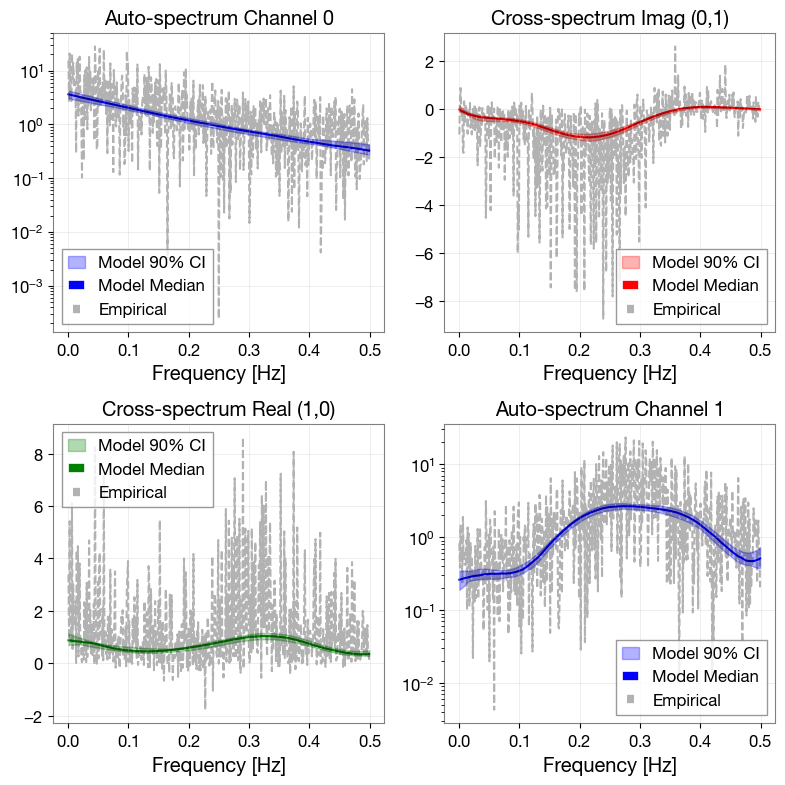
\includegraphics[width=.85\linewidth]{figures/var2_simulation.png}
    \caption{VAR2}
    \label{fig:placeholder}
\end{figure}



Following Liu et at, we simulate 500 independent realisations of a bivariate time series from a vector autoregressive model of order 2, VAR(2), using three  different sample sizes $n=256;512;1024$ (refer to \citet[Section~4.2,][]{Liu2023} for the definitions of the VAR(2) models).
The spectral densities are estimated using both the Pspline, SGVB method and \citet{Liu2023}'s vectorized nonparametrically corrected method (VNPC), an MCMC-based approach that samples from the exact posterior distribution without a variational approximation\footnote{For the VNPC analyses, we use the software and settings provided by \citet{Liu2023}, specific for the VAR(2) models.}.
We validate the multivariate P-spline method using synthetic data from Vector Autoregressive (VAR) processes with known theoretical spectral properties. 
The theoretical spectral density matrix provides exact ground truth for comparison.



Figure~\ref{fig:var_simulation} shows results for bivariate VAR(2) data. 
The P-spline estimates accurately recover both auto-spectral components (diagonal elements) and cross-spectral components (off-diagonal real and imaginary parts). 
The posterior medians track the XYZ. 
The 90\% credible intervals demonstrate appropriate uncertainty quantification across all spectral components.

Quantitative assessment reveals mean squared errors of $XYZ$ for auto-spectral estimates and $XYZ$ for cross-spectral estimates relative to theoretical values. 
Coverage probabilities for credible intervals exceed $XY\%$ across all frequencies


\begin{figure}
    \centering
    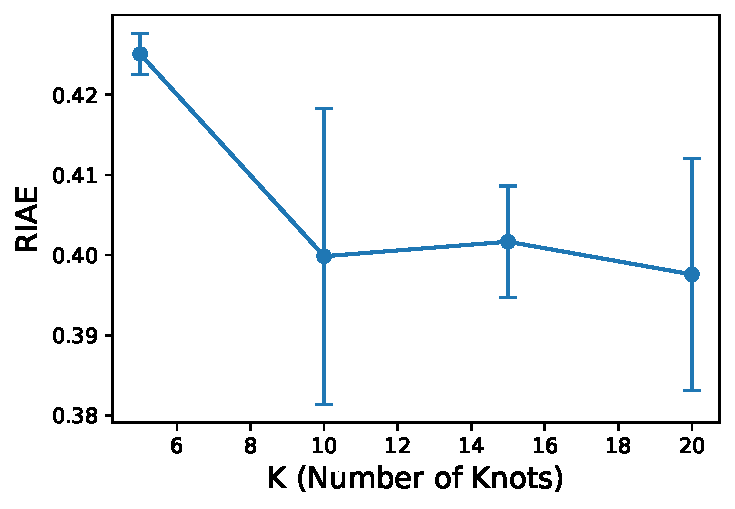
\includegraphics[width=1\linewidth]{figures/riae_vs_K.pdf}
    \caption{RIAE vs K}
    \label{fig:riae_vs_k}
\end{figure}
\begin{figure}
    \centering
    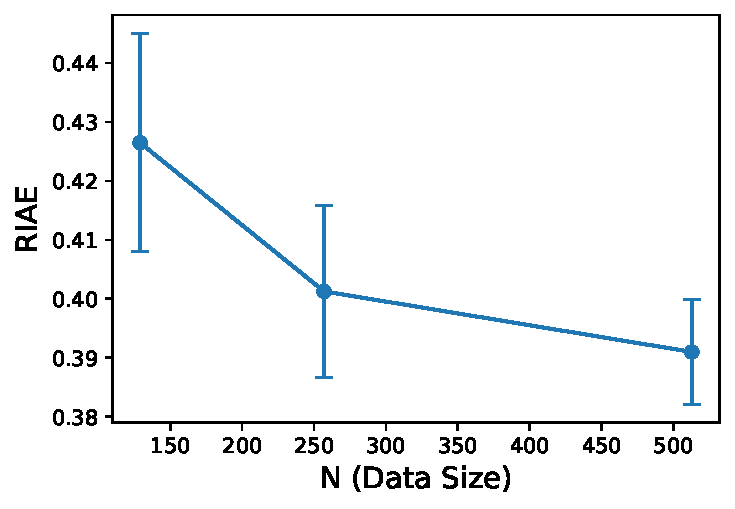
\includegraphics[width=1\linewidth]{figures/riae_vs_N.pdf}
    \caption{RIAE vs N}
    \label{fig:riae_vs_n}
\end{figure}



\subsection{LISA }
\begin{figure}
    \centering
    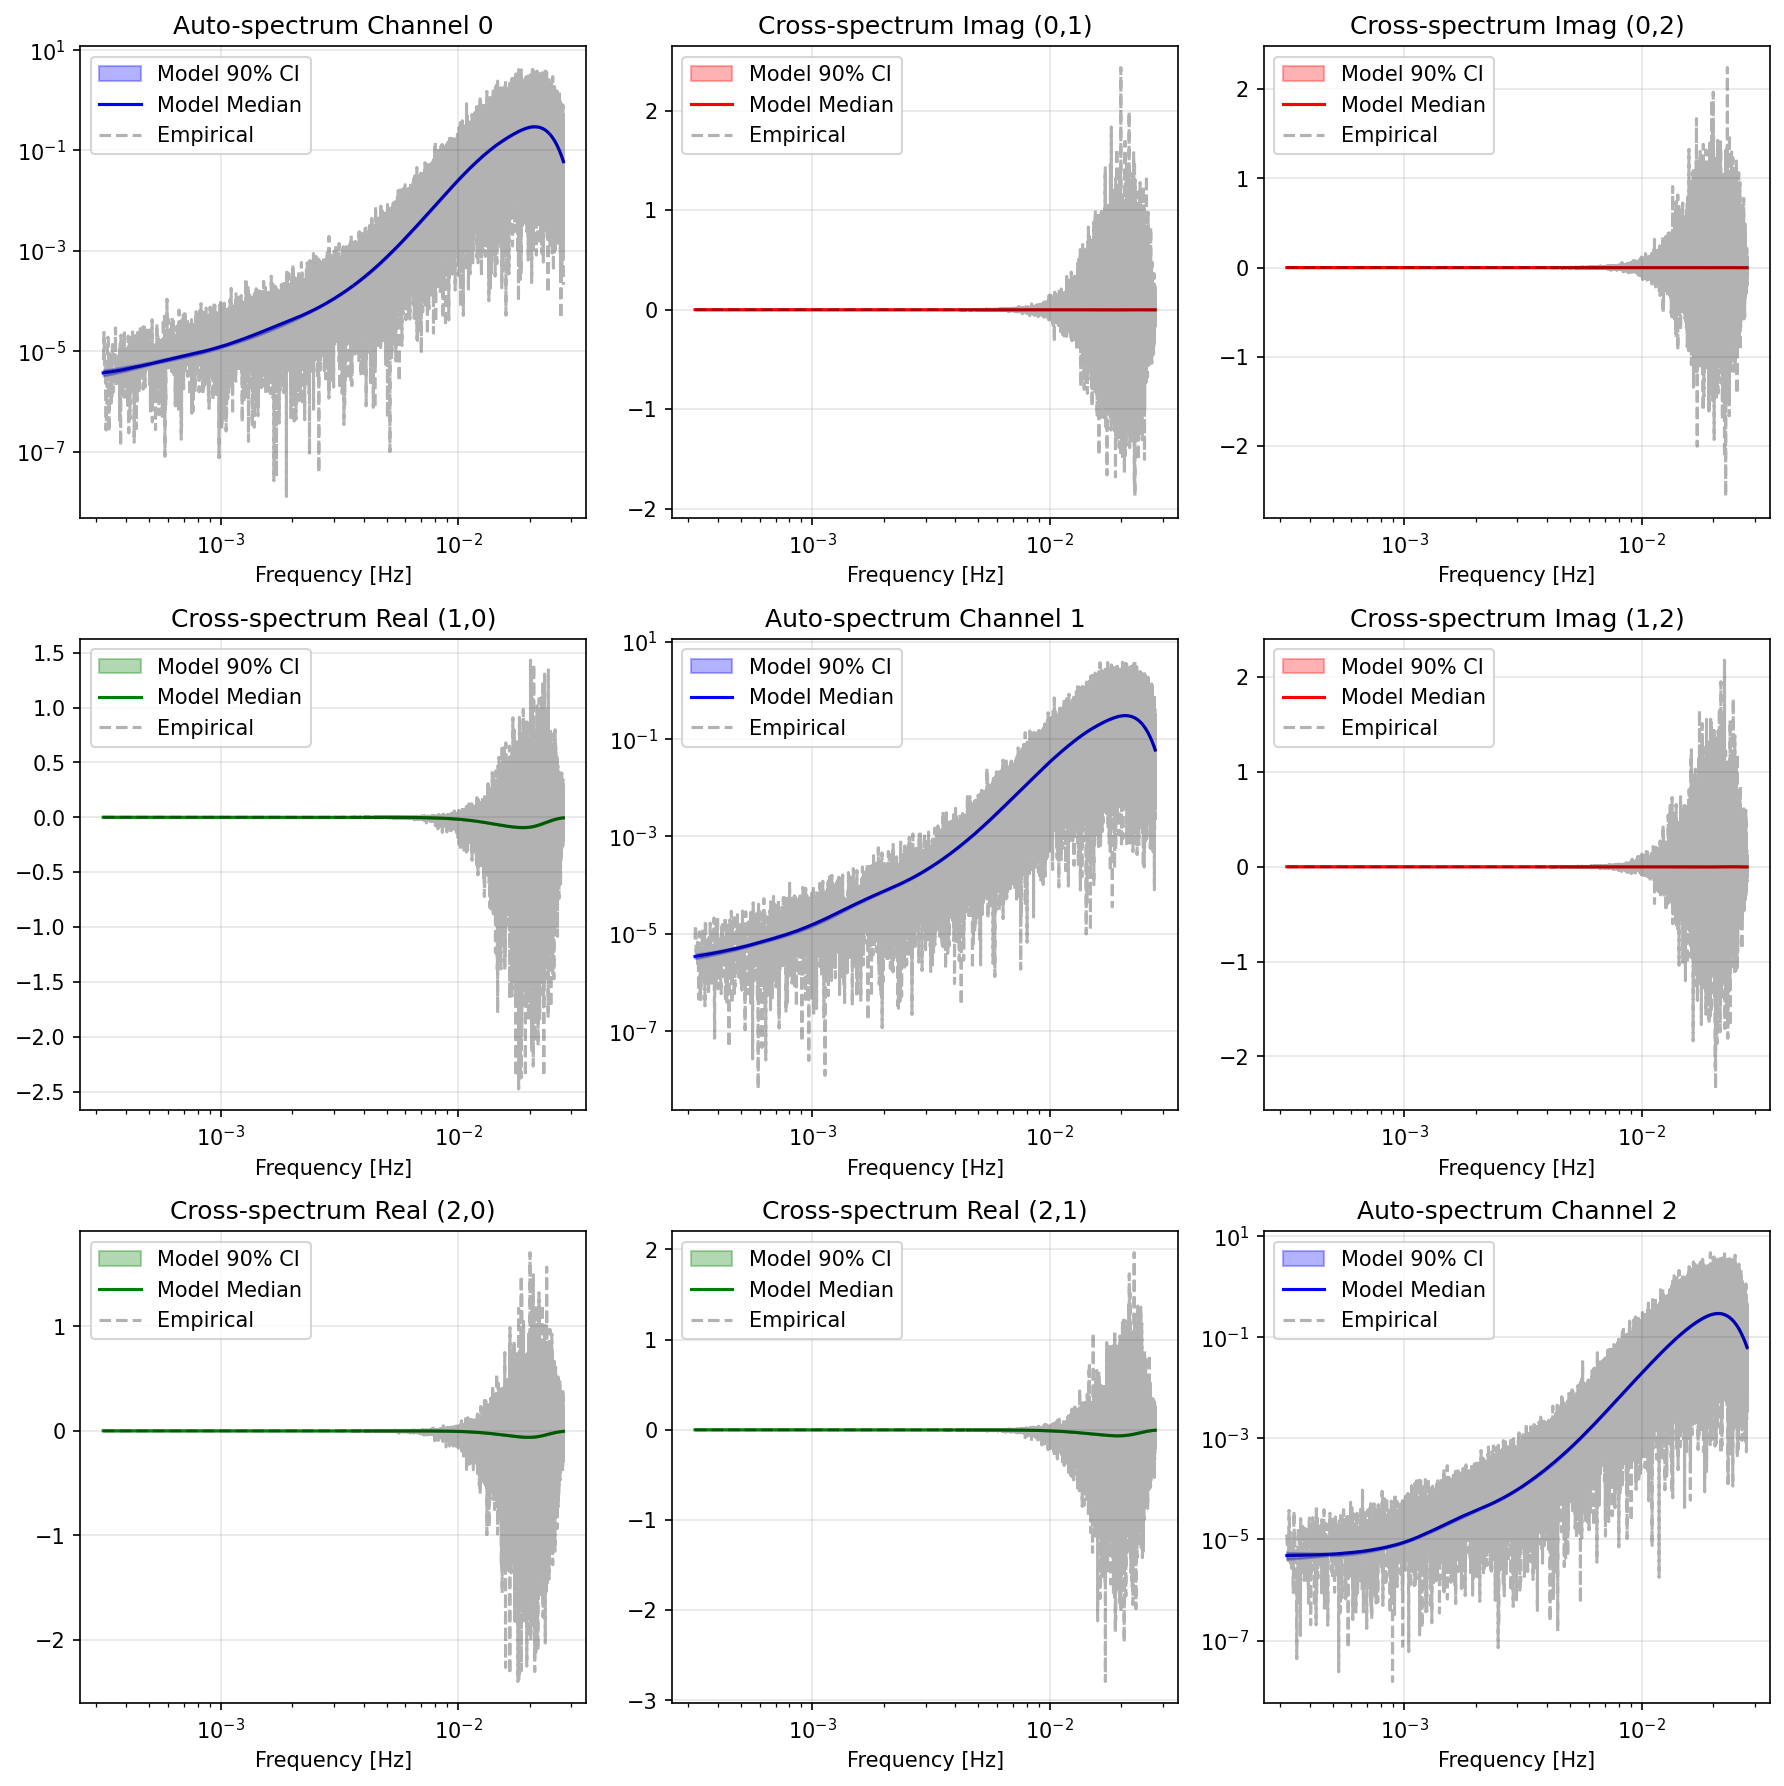
\includegraphics[width=1\linewidth]{figures/lisa.png}
    \caption{LISA work in prog}
    \label{fig:placeholder}
\end{figure}

Notes from jonathan gair



\section*{Implementation}
\begin{onecolumn}
\begin{lstlisting}[style=pythonstyle]
@jax.jit
def whittle_likelihood_arrays(
    y_re: jnp.ndarray,
    y_im: jnp.ndarray,
    Z_re: jnp.ndarray,
    Z_im: jnp.ndarray,
    log_delta_sq: jnp.ndarray,   # (n_freq, n_dim)
    theta_re: jnp.ndarray,       # (n_freq, n_theta)
    theta_im: jnp.ndarray        # (n_freq, n_theta)
) -> jnp.ndarray:
    """Multivariate Whittle likelihood for Cholesky PSD parameterization - JIT version."""
    sum_log_det = -jnp.sum(log_delta_sq)
    exp_neg_log_delta = jnp.exp(-log_delta_sq)

    if Z_re.shape[2] > 0:
        Z_theta_re = jnp.einsum('fij,fj->fi', Z_re, theta_re) - jnp.einsum('fij,fj->fi', Z_im, theta_im)
        Z_theta_im = jnp.einsum('fij,fj->fi', Z_re, theta_im) + jnp.einsum('fij,fj->fi', Z_im, theta_re)
        u_re = y_re - Z_theta_re
        u_im = y_im - Z_theta_im
    else:
        u_re = y_re
        u_im = y_im

    numerator = u_re ** 2 + u_im ** 2
    internal = numerator * exp_neg_log_delta
    tmp2 = -jnp.sum(internal)
    return sum_log_det + tmp2


def multivariate_psplines_model(
    y_re: jnp.ndarray,       # FFT real parts
    y_im: jnp.ndarray,       # FFT imaginary parts
    Z_re: jnp.ndarray,       # Design matrix real parts
    Z_im: jnp.ndarray,       # Design matrix imaginary parts
    all_bases,               # List of basis matrices
    all_penalties,           # List of penalty matrices
    alpha_phi: float = 1.0,
    beta_phi: float = 1.0,
    alpha_delta: float = 1e-4,
    beta_delta: float = 1e-4,
):
    """
    NumPyro model for multivariate PSD estimation using P-splines and Cholesky parameterization.
    """
    # Extract dimensions from input arrays (these are static during compilation)
    n_freq, n_dim = y_re.shape
    n_theta = Z_re.shape[2]

    component_idx = 0
    log_delta_components = []

    # Initialize total log prior accumulator
    log_prior_total = jnp.array(0.0)

    # Diagonal components (one per channel)
    for j in range(n_dim):  # Now n_dim is a concrete Python int
        delta = numpyro.sample(f"delta_{j}", dist.Gamma(alpha_delta, beta_delta))
        phi = numpyro.sample(f"phi_delta_{j}", dist.Gamma(alpha_phi, delta * beta_phi))

        k = all_penalties[component_idx].shape[0]
        weights = numpyro.sample(f"weights_delta_{j}", dist.Normal(0, 1).expand((k,)).to_event(1))

        # Prior factor for weights
        wPw = jnp.dot(weights, jnp.dot(all_penalties[component_idx], weights))
        log_prior_w = 0.5 * k * jnp.log(phi) - 0.5 * phi * wPw
        numpyro.factor(f"weights_prior_delta_{j}", log_prior_w)
        log_prior_total += log_prior_w

        # Compute log diagonal element
        log_delta_sq_j = all_bases[component_idx] @ weights
        log_delta_components.append(log_delta_sq_j)
        component_idx += 1

    log_delta_sq = jnp.stack(log_delta_components, axis=1)

    # Off-diagonal components (if multivariate)
    if n_theta > 0:
        # Real part of off-diagonal terms
        delta_re = numpyro.sample("delta_theta_re", dist.Gamma(alpha_delta, beta_delta))
        phi_re = numpyro.sample("phi_theta_re", dist.Gamma(alpha_phi, delta_re * beta_phi))

        k = all_penalties[component_idx].shape[0]
        weights_re = numpyro.sample("weights_theta_re", dist.Normal(0, 1).expand((k,)).to_event(1))

        wPw_re = jnp.dot(weights_re, jnp.dot(all_penalties[component_idx], weights_re))
        log_prior_w_re = 0.5 * k * jnp.log(phi_re) - 0.5 * phi_re * wPw_re
        numpyro.factor("weights_prior_theta_re", log_prior_w_re)
        log_prior_total += log_prior_w_re

        theta_re_base = all_bases[component_idx] @ weights_re
        theta_re = jnp.tile(theta_re_base[:, None], (1, max(1, n_theta)))
        component_idx += 1

        # Imaginary part of off-diagonal terms
        delta_im = numpyro.sample("delta_theta_im", dist.Gamma(alpha_delta, beta_delta))
        phi_im = numpyro.sample("phi_theta_im", dist.Gamma(alpha_phi, delta_im * beta_phi))

        k = all_penalties[component_idx].shape[0]
        weights_im = numpyro.sample("weights_theta_im", dist.Normal(0, 1).expand((k,)).to_event(1))

        wPw_im = jnp.dot(weights_im, jnp.dot(all_penalties[component_idx], weights_im))
        log_prior_w_im = 0.5 * k * jnp.log(phi_im) - 0.5 * phi_im * wPw_im
        numpyro.factor("weights_prior_theta_im", log_prior_w_im)
        log_prior_total += log_prior_w_im

        theta_im_base = all_bases[component_idx] @ weights_im
        theta_im = jnp.tile(theta_im_base[:, None], (1, max(1, n_theta)))
    else:
        theta_re = jnp.zeros((n_freq, 0))
        theta_im = jnp.zeros((n_freq, 0))

    # Likelihood using individual arrays
    log_likelihood = whittle_likelihood_arrays(
        y_re, y_im, Z_re, Z_im, log_delta_sq, theta_re, theta_im
    )
    numpyro.factor("likelihood", log_likelihood)

    # Store deterministic quantities for diagnostics
    numpyro.deterministic("lp", log_prior_total + log_likelihood)
    numpyro.deterministic("log_delta_sq", log_delta_sq)
    numpyro.deterministic("theta_re", theta_re)
    numpyro.deterministic("theta_im", theta_im)
    numpyro.deterministic("log_likelihood", log_likelihood)
\end{lstlisting}

\end{onecolumn}


\section{Discussion}


\begin{acknowledgments}

\end{acknowledgments}


\bibliography{apssamp}% Produces the bibliography via BibTeX.

\end{document}
%
% ****** End of file apssamp.tex ******
